% Created by tikzDevice version 0.12.3.1 on 2021-04-09 22:35:57
% !TEX encoding = UTF-8 Unicode
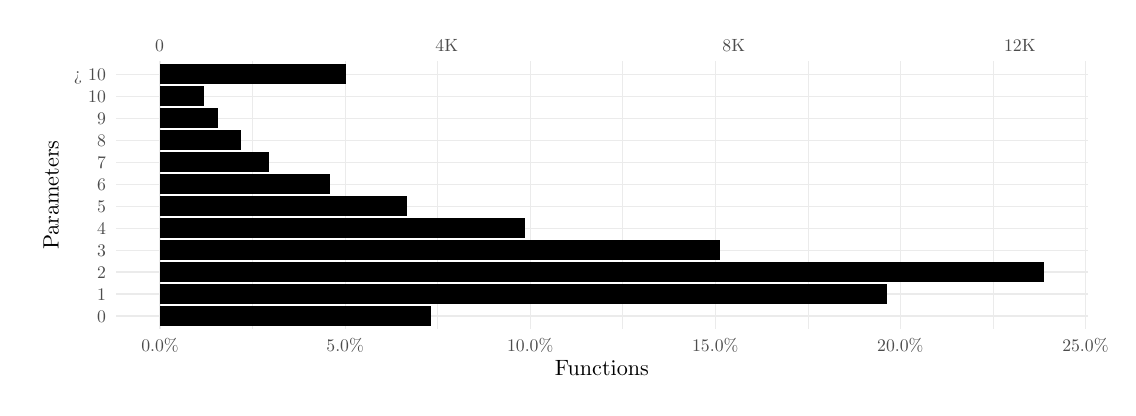
\begin{tikzpicture}[x=1pt,y=1pt]
\definecolor{fillColor}{RGB}{255,255,255}
\path[use as bounding box,fill=fillColor,fill opacity=0.00] (0,0) rectangle (390.26,130.09);
\begin{scope}
\path[clip] ( 31.86, 21.16) rectangle (383.14,117.99);
\definecolor{drawColor}{gray}{0.92}

\path[draw=drawColor,line width= 0.2pt,line join=round] ( 81.27, 21.16) --
	( 81.27,117.99);

\path[draw=drawColor,line width= 0.2pt,line join=round] (148.15, 21.16) --
	(148.15,117.99);

\path[draw=drawColor,line width= 0.2pt,line join=round] (215.02, 21.16) --
	(215.02,117.99);

\path[draw=drawColor,line width= 0.2pt,line join=round] (281.90, 21.16) --
	(281.90,117.99);

\path[draw=drawColor,line width= 0.2pt,line join=round] (348.77, 21.16) --
	(348.77,117.99);

\path[draw=drawColor,line width= 0.4pt,line join=round] ( 31.86, 25.92) --
	(383.14, 25.92);

\path[draw=drawColor,line width= 0.4pt,line join=round] ( 31.86, 33.86) --
	(383.14, 33.86);

\path[draw=drawColor,line width= 0.4pt,line join=round] ( 31.86, 41.80) --
	(383.14, 41.80);

\path[draw=drawColor,line width= 0.4pt,line join=round] ( 31.86, 49.73) --
	(383.14, 49.73);

\path[draw=drawColor,line width= 0.4pt,line join=round] ( 31.86, 57.67) --
	(383.14, 57.67);

\path[draw=drawColor,line width= 0.4pt,line join=round] ( 31.86, 65.61) --
	(383.14, 65.61);

\path[draw=drawColor,line width= 0.4pt,line join=round] ( 31.86, 73.54) --
	(383.14, 73.54);

\path[draw=drawColor,line width= 0.4pt,line join=round] ( 31.86, 81.48) --
	(383.14, 81.48);

\path[draw=drawColor,line width= 0.4pt,line join=round] ( 31.86, 89.42) --
	(383.14, 89.42);

\path[draw=drawColor,line width= 0.4pt,line join=round] ( 31.86, 97.35) --
	(383.14, 97.35);

\path[draw=drawColor,line width= 0.4pt,line join=round] ( 31.86,105.29) --
	(383.14,105.29);

\path[draw=drawColor,line width= 0.4pt,line join=round] ( 31.86,113.23) --
	(383.14,113.23);

\path[draw=drawColor,line width= 0.4pt,line join=round] ( 47.83, 21.16) --
	( 47.83,117.99);

\path[draw=drawColor,line width= 0.4pt,line join=round] (114.71, 21.16) --
	(114.71,117.99);

\path[draw=drawColor,line width= 0.4pt,line join=round] (181.58, 21.16) --
	(181.58,117.99);

\path[draw=drawColor,line width= 0.4pt,line join=round] (248.46, 21.16) --
	(248.46,117.99);

\path[draw=drawColor,line width= 0.4pt,line join=round] (315.34, 21.16) --
	(315.34,117.99);

\path[draw=drawColor,line width= 0.4pt,line join=round] (382.21, 21.16) --
	(382.21,117.99);
\definecolor{fillColor}{RGB}{0,0,0}

\path[fill=fillColor] ( 47.83,109.66) rectangle (115.04,116.80);

\path[fill=fillColor] ( 47.83, 22.35) rectangle (145.68, 29.50);

\path[fill=fillColor] ( 47.83, 30.29) rectangle (310.59, 37.43);

\path[fill=fillColor] ( 47.83,101.72) rectangle ( 63.63,108.86);

\path[fill=fillColor] ( 47.83, 38.23) rectangle (367.18, 45.37);

\path[fill=fillColor] ( 47.83, 46.16) rectangle (250.08, 53.31);

\path[fill=fillColor] ( 47.83, 54.10) rectangle (179.66, 61.24);

\path[fill=fillColor] ( 47.83, 62.04) rectangle (137.11, 69.18);

\path[fill=fillColor] ( 47.83, 69.97) rectangle (109.42, 77.12);

\path[fill=fillColor] ( 47.83, 77.91) rectangle ( 87.10, 85.05);

\path[fill=fillColor] ( 47.83, 85.85) rectangle ( 77.25, 92.99);

\path[fill=fillColor] ( 47.83, 93.78) rectangle ( 68.76,100.93);
\end{scope}
\begin{scope}
\path[clip] (  0.00,  0.00) rectangle (390.26,130.09);
\definecolor{drawColor}{gray}{0.30}

\node[text=drawColor,anchor=base,inner sep=0pt, outer sep=0pt, scale=  0.64] at ( 47.69,121.59) {0};

\node[text=drawColor,anchor=base,inner sep=0pt, outer sep=0pt, scale=  0.64] at (151.42,121.59) {4K};

\node[text=drawColor,anchor=base,inner sep=0pt, outer sep=0pt, scale=  0.64] at (255.15,121.59) {8K};

\node[text=drawColor,anchor=base,inner sep=0pt, outer sep=0pt, scale=  0.64] at (358.53,121.59) {12K};
\end{scope}
\begin{scope}
\path[clip] (  0.00,  0.00) rectangle (390.26,130.09);
\definecolor{drawColor}{gray}{0.30}

\node[text=drawColor,anchor=base east,inner sep=0pt, outer sep=0pt, scale=  0.64] at ( 28.26, 23.72) {0};

\node[text=drawColor,anchor=base east,inner sep=0pt, outer sep=0pt, scale=  0.64] at ( 28.26, 31.66) {1};

\node[text=drawColor,anchor=base east,inner sep=0pt, outer sep=0pt, scale=  0.64] at ( 28.26, 39.59) {2};

\node[text=drawColor,anchor=base east,inner sep=0pt, outer sep=0pt, scale=  0.64] at ( 28.26, 47.53) {3};

\node[text=drawColor,anchor=base east,inner sep=0pt, outer sep=0pt, scale=  0.64] at ( 28.26, 55.47) {4};

\node[text=drawColor,anchor=base east,inner sep=0pt, outer sep=0pt, scale=  0.64] at ( 28.26, 63.40) {5};

\node[text=drawColor,anchor=base east,inner sep=0pt, outer sep=0pt, scale=  0.64] at ( 28.26, 71.34) {6};

\node[text=drawColor,anchor=base east,inner sep=0pt, outer sep=0pt, scale=  0.64] at ( 28.26, 79.28) {7};

\node[text=drawColor,anchor=base east,inner sep=0pt, outer sep=0pt, scale=  0.64] at ( 28.26, 87.21) {8};

\node[text=drawColor,anchor=base east,inner sep=0pt, outer sep=0pt, scale=  0.64] at ( 28.26, 95.15) {9};

\node[text=drawColor,anchor=base east,inner sep=0pt, outer sep=0pt, scale=  0.64] at ( 28.26,103.09) {10};

\node[text=drawColor,anchor=base east,inner sep=0pt, outer sep=0pt, scale=  0.64] at ( 28.26,111.02) {> 10};
\end{scope}
\begin{scope}
\path[clip] (  0.00,  0.00) rectangle (390.26,130.09);
\definecolor{drawColor}{gray}{0.30}

\node[text=drawColor,anchor=base,inner sep=0pt, outer sep=0pt, scale=  0.64] at ( 47.83, 13.15) {0.0{\%}};

\node[text=drawColor,anchor=base,inner sep=0pt, outer sep=0pt, scale=  0.64] at (114.71, 13.15) {5.0{\%}};

\node[text=drawColor,anchor=base,inner sep=0pt, outer sep=0pt, scale=  0.64] at (181.58, 13.15) {10.0{\%}};

\node[text=drawColor,anchor=base,inner sep=0pt, outer sep=0pt, scale=  0.64] at (248.46, 13.15) {15.0{\%}};

\node[text=drawColor,anchor=base,inner sep=0pt, outer sep=0pt, scale=  0.64] at (315.34, 13.15) {20.0{\%}};

\node[text=drawColor,anchor=base,inner sep=0pt, outer sep=0pt, scale=  0.64] at (382.21, 13.15) {25.0{\%}};
\end{scope}
\begin{scope}
\path[clip] (  0.00,  0.00) rectangle (390.26,130.09);
\definecolor{drawColor}{RGB}{0,0,0}

\node[text=drawColor,anchor=base,inner sep=0pt, outer sep=0pt, scale=  0.80] at (207.50,  4.40) {Functions};
\end{scope}
\begin{scope}
\path[clip] (  0.00,  0.00) rectangle (390.26,130.09);
\definecolor{drawColor}{RGB}{0,0,0}

\node[text=drawColor,rotate= 90.00,anchor=base,inner sep=0pt, outer sep=0pt, scale=  0.80] at ( 11.20, 69.58) {Parameters};
\end{scope}
\end{tikzpicture}
